% Comments start with % (percent) character and last till the end of the line.
%
% The line below tells TeXworks editor to use pdflatex for compilation
% of this document; remove it if you want to use another engine 
%
%!TEX program = pdflatex
%
% LaTeX2e document starts with \documentclass[options]{<class-name>}
% <class-name> can be one of the standard LaTeX document classes: 
% article, report or book, or some other specialised class.
%
\documentclass[twocolumn]{article}
%
% Preamble of LaTeX document is everything before \begin{document}.
% Preamble is used to load extension packages and to set up global 
% parameters and configuration for the entire document.
%
% Extension packages providing additional functionality
\usepackage{amsmath}       % additional math environments
\usepackage{amsfonts}
\usepackage{graphicx}      % graphics import from external files 
\usepackage{epstopdf}      % automates .eps to .pdf conversion 
% epstopdf package may require --shell-escape option to pdflatex
\usepackage{booktabs}      % table typesetting additions
\usepackage{siunitx}       % number and units formatting
\usepackage{caption}       % customisation of captions
\usepackage{url}           % format url addresses
\usepackage{abstract}		% allows formatting of abstract
%\usepackage{tikz,pgfplots} % diagrams and data plots
%
% set up caption options
\captionsetup{margin=12pt,font=small,labelfont=bf}
%
%removes abstract title
\renewcommand{\abstractname}{}
%sets abstract margins
\setlength{\absleftindent}{30mm}
\setlength{\absrightindent}{30mm}
%
% global options for siunitx
%\sisetup{seperr,repeatunits=false,per=symbol}
%
% some handy commands for referencing;
% the optional argument overrides the default label, e.g.
% \figref[FIG.~]{fig:label}
\newcommand{\figref}[2][\figurename~]{#1\ref{#2}}
\newcommand{\tabref}[2][\tablename~]{#1\ref{#2}}
\newcommand{\secref}[2][Section~]{#1\ref{#2}}


% The document content starts with \begin{document} 
% and is finished with \end{document}
%
\begin{document}
\title{MPhys Final Project Report} % fill in the title here
\author{Andrew Morris}% fill in your name here
\date{March 2015} % date of the report
\twocolumn[	% makes title and abstract appear over entire page width
\maketitle % formats the title

\begin{onecolabstract}
\noindent
My Abstract 
\tableofcontents
\end{onecolabstract}
\vspace{5 mm}
]

\section{Introduction}
\label{sec:Introduction}

1. Interest and importance of thermoelectricity. \newline
2. Choose material (Si-Ge). \newline
3. Calculate ZT. \newline
4. Check calculations consistent with Chen. \newline
5. Extend calculations (EMA, specularity...) \newline
6. Suggest new research. \newline

\subsection{Thermoelectric History}
\label{sec:Thermoelectric History}
Histpry of thermoelectric effect. Who found what when.

\subsection{Thermoelectric Generators}
\label{sec:Thermoelectric Generators}
A schematic generator:
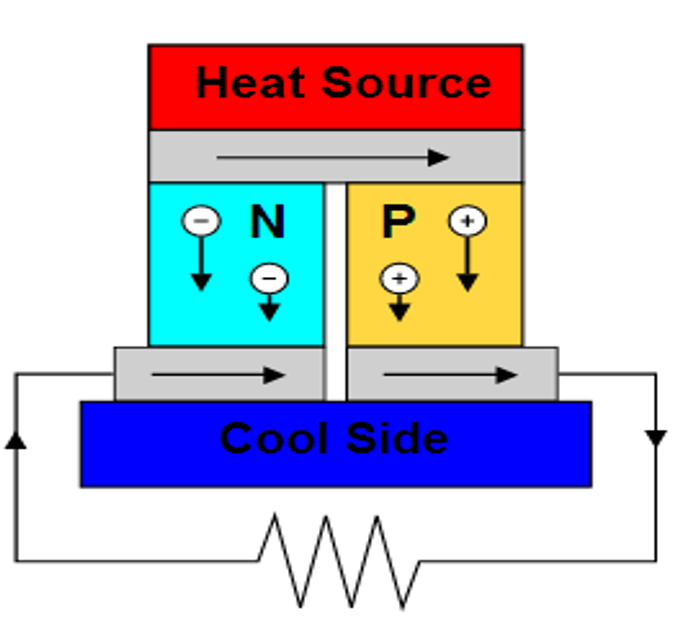
\includegraphics[width=80mm]{schematic_generator.png}Can use generators using thermoelectric effect in places where maintenance is difficult and total power requirements low, for example in space.



A common RTG (radioisotope thermoelectric generator) application is spacecraft power supply. RTGs were used for probes that traveled far from the Sun where the radiation wastoo weak for photo-voltaic solar panels. they were used on the Voyager spacecraft: 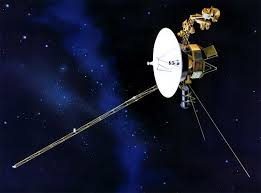
\includegraphics[width=80mm]{voyager.jpg}

\subsection{Thermoelectric Efficiency}
\label{sec:Thermoelectric Efficiency}
Thermoelectric efficiency - retaionship with Carnot efficiency. Defintion of $\mathbf{ZT}$

\subsection{Thermoelectric Materiasls}
\label{sec:Thermoelectric Materials}
Required properties. Temperature range. Need models to guide manufacturing because making them is expensive. Reports of other groups (Chen). Silicon-germanium looks interesting. Nano composites perform better than alloys.
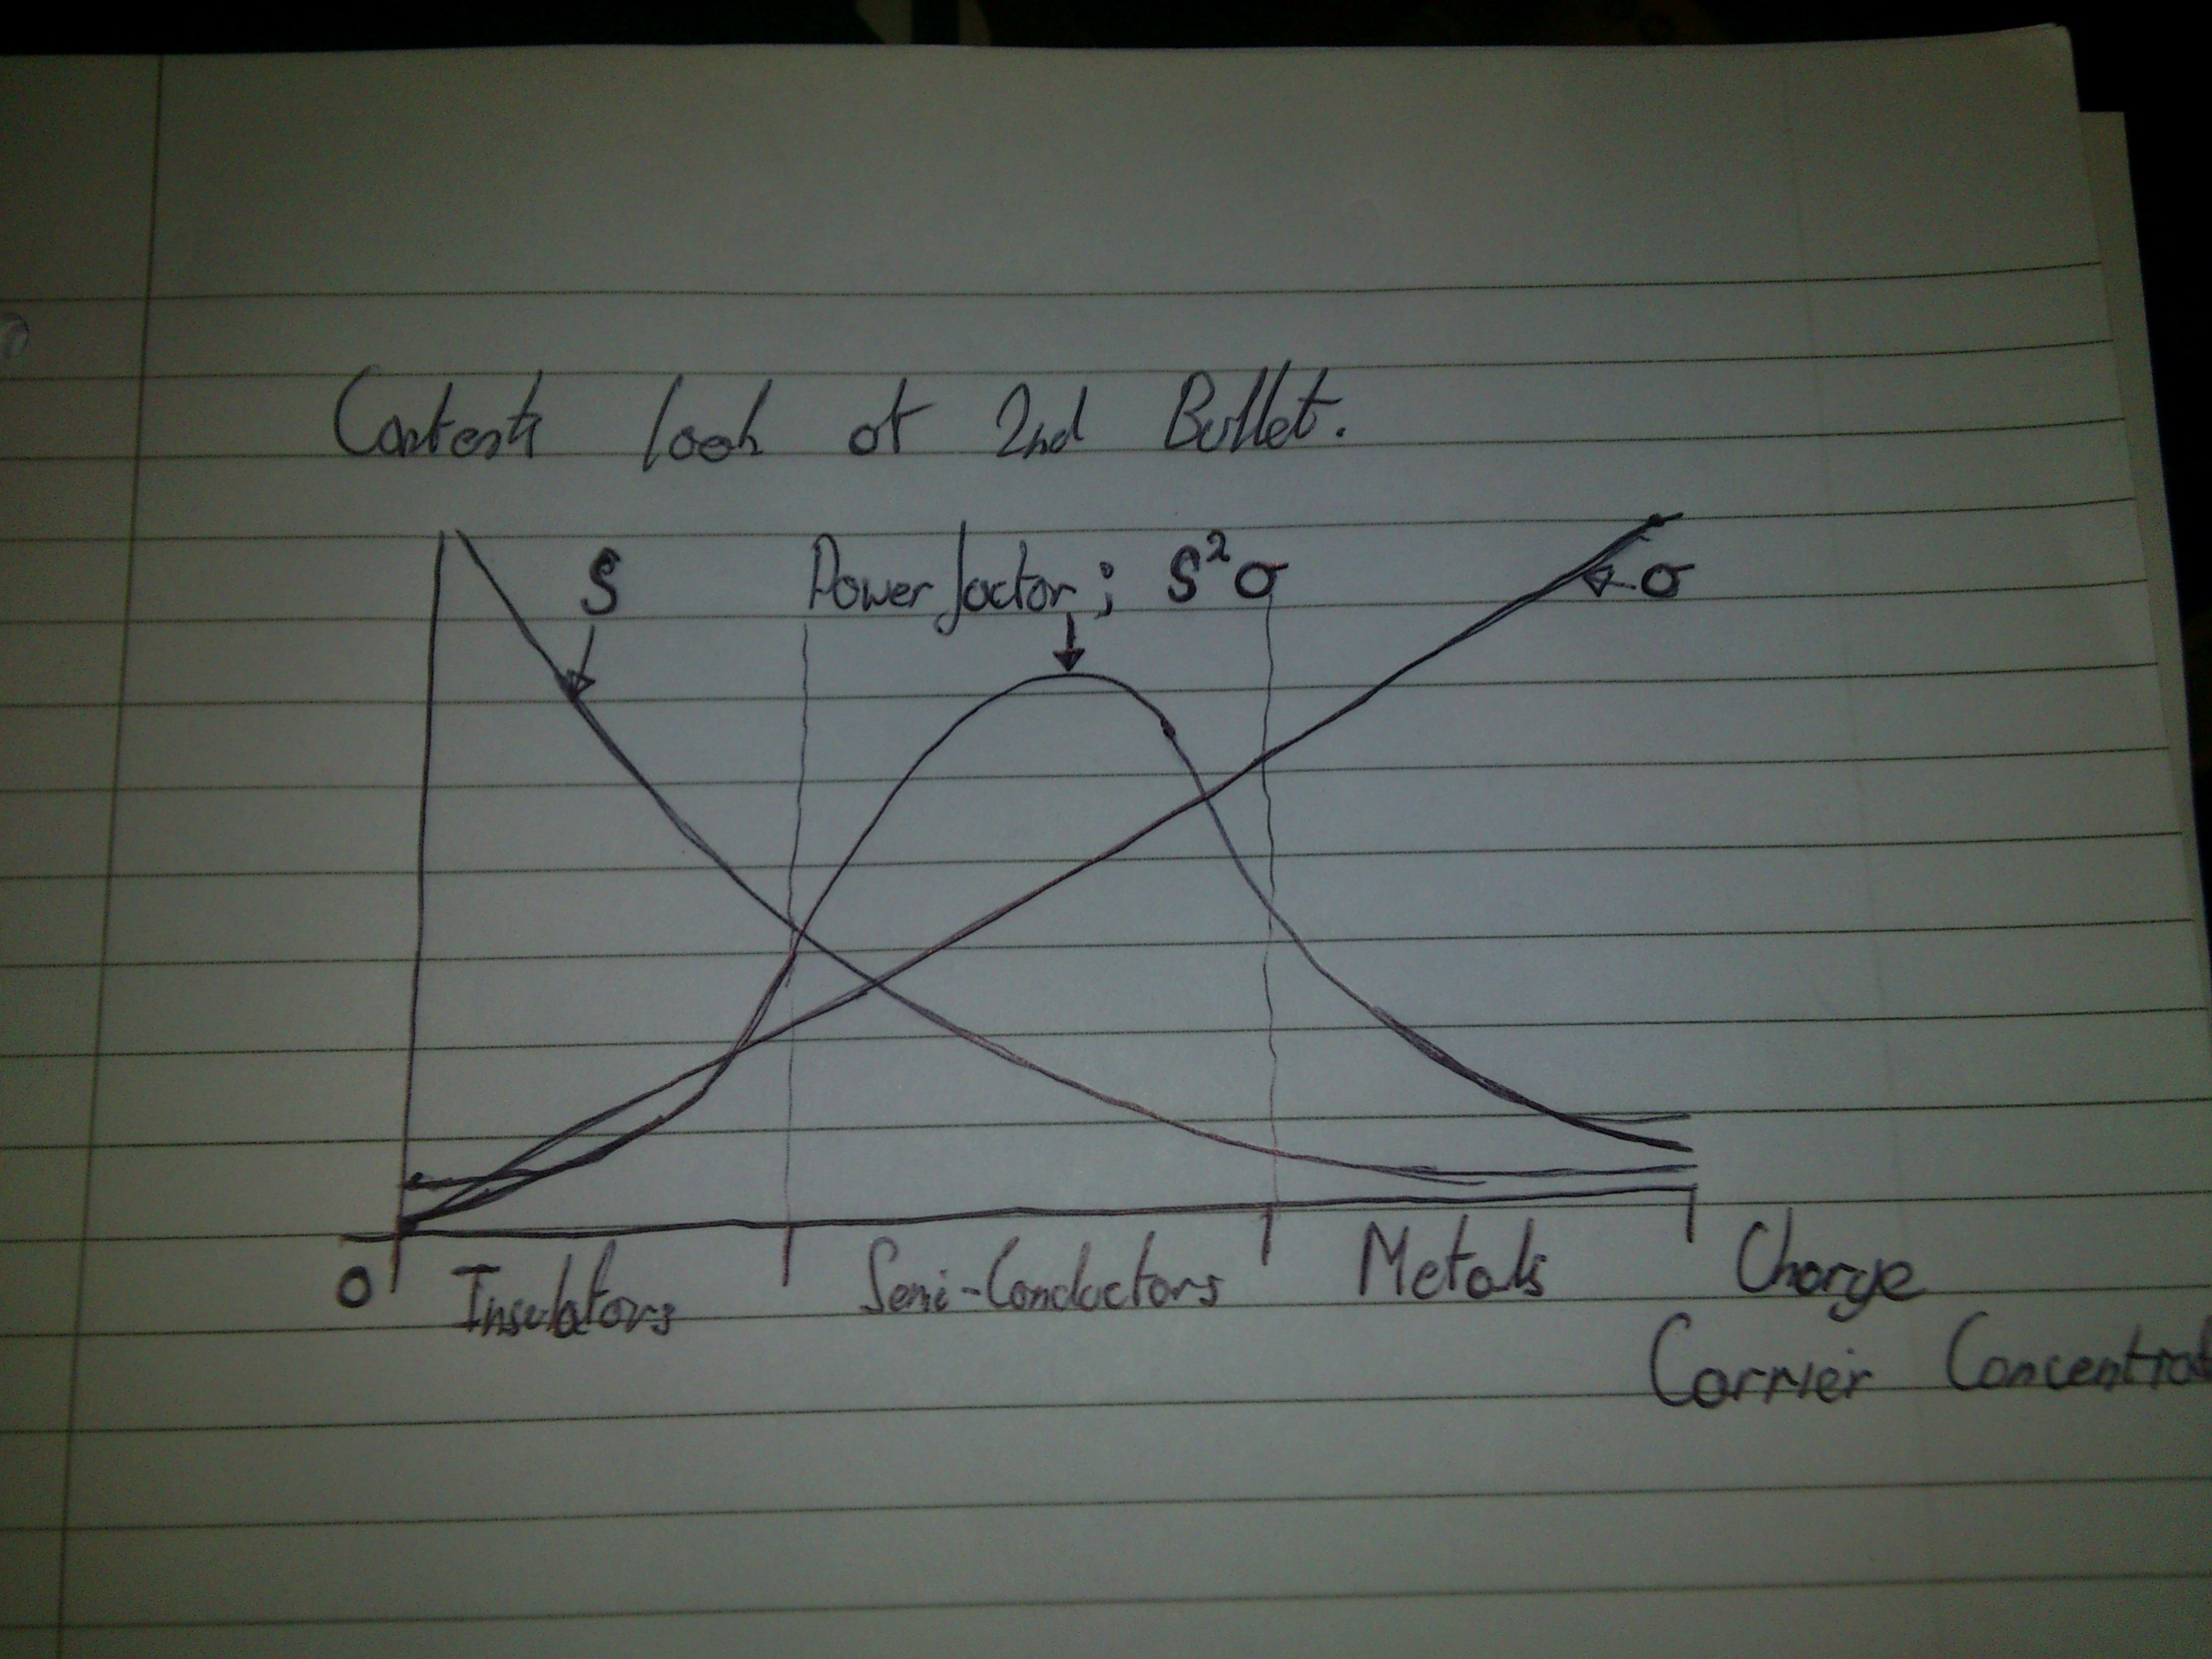
\includegraphics[width=80mm]{Roughpowerfactor.jpg}
\includegraphics[width=80mm]{kphindependentofcc.jpg}
\includegraphics[width=80mm]{ZTvsccc.jpg}
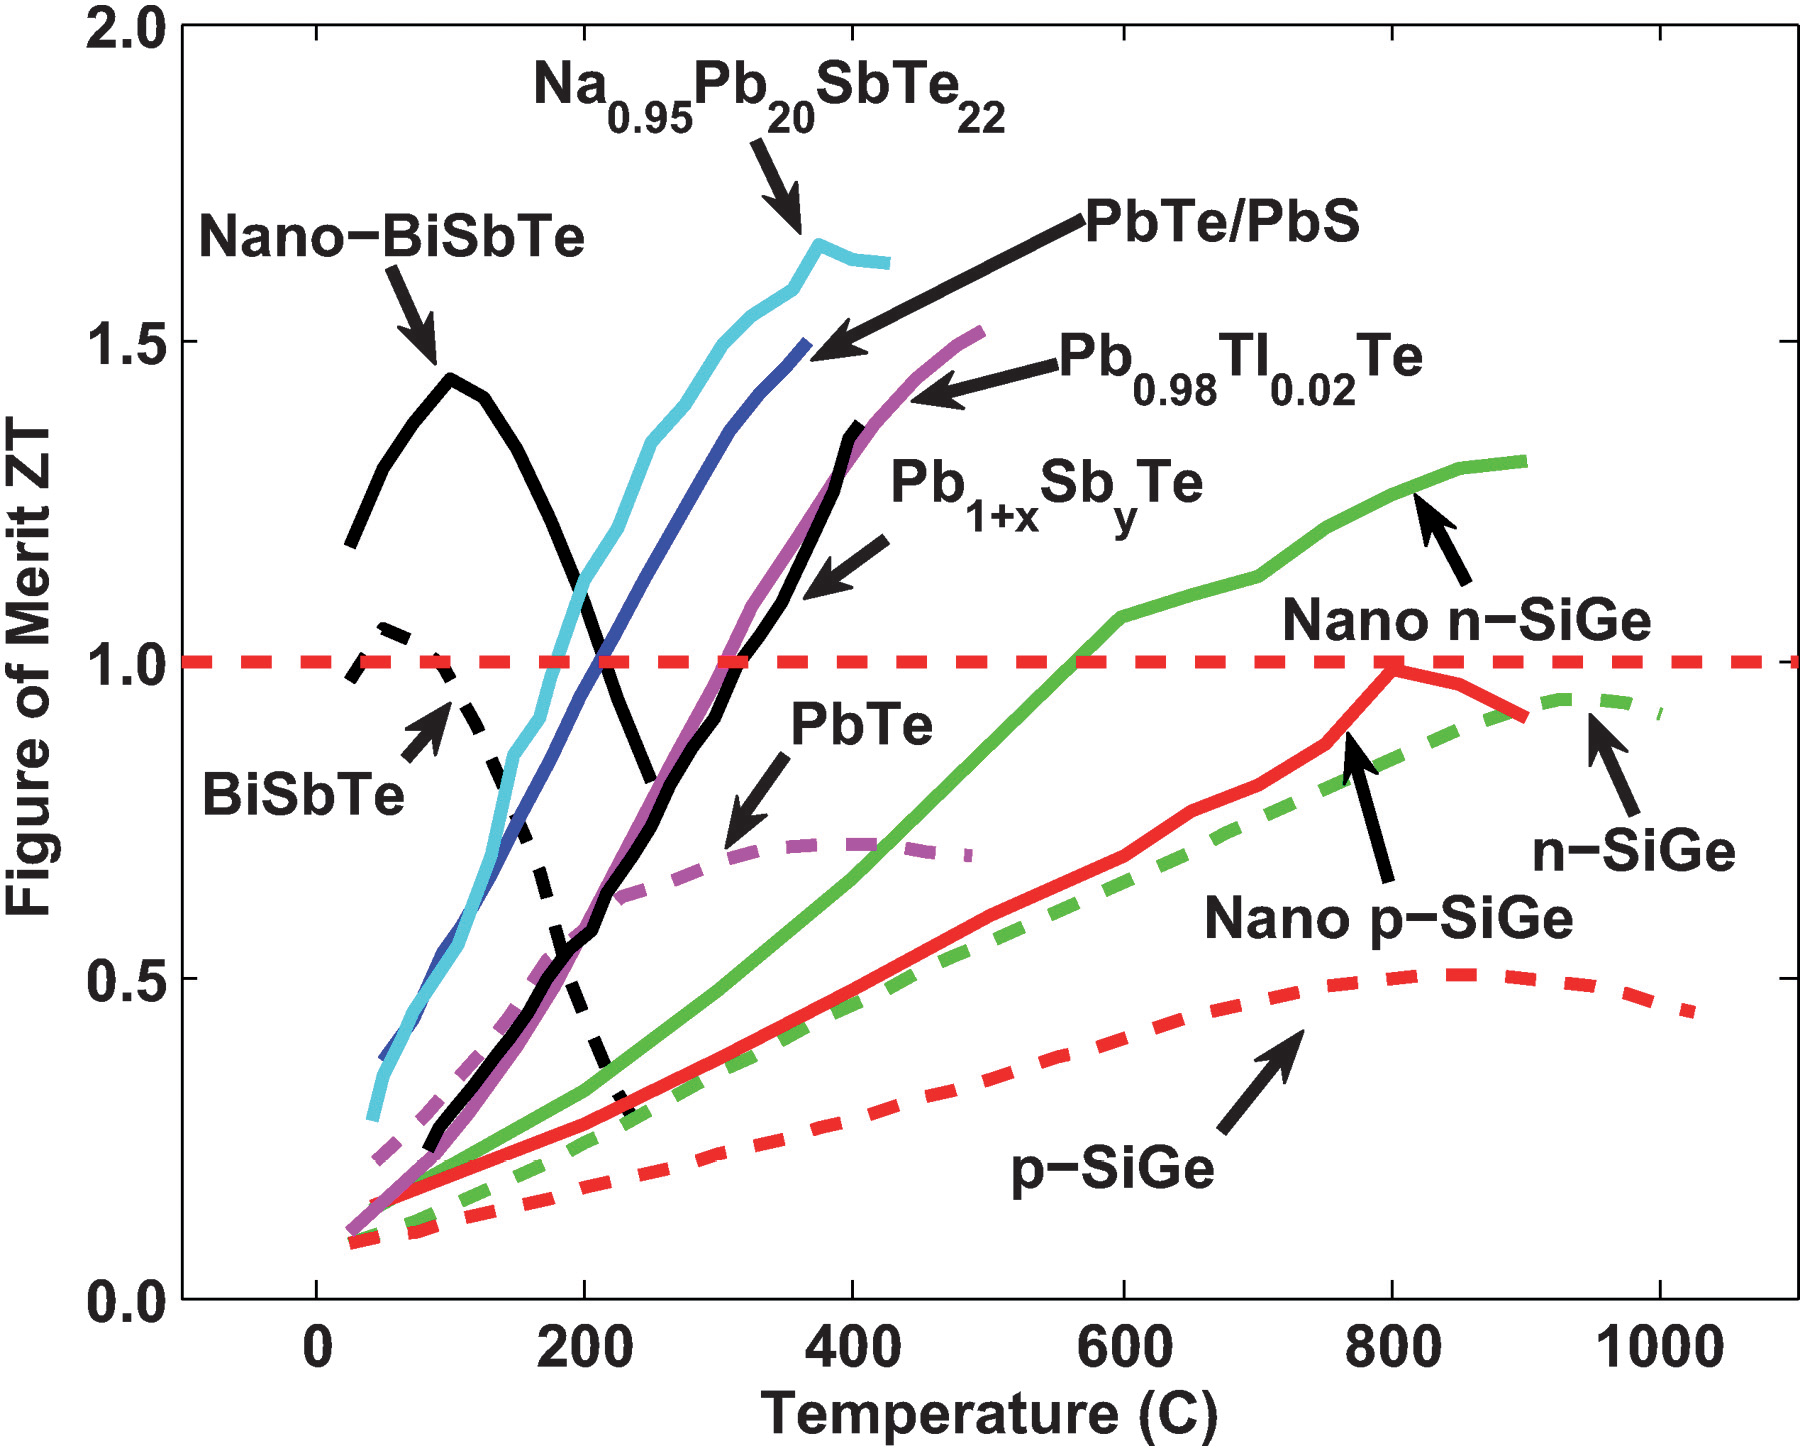
\includegraphics[width=80mm]{Chen.png}

\section{Modelling $\mathbf{ZT}$ }
\label{sec:Modelling ZT}

\subsection{Components of $\mathbf{ZT}$}
\label{sec:Components of ZT}

\subsubsection{Power Factor}
\label{sec:Power Factor}
Seebeck effect. Electrical conuductivity. Electron mean free path. Loks like cyrstal to electrons,


\subsubsection{Thermal Conductivity}
\label{sec:Thermal Conductivity}
Contributions to thermal conductivity. Weideman Franz law. Electrob thermal conductivity related to electrical conductivty. Leaves only phone component to mimiimize. Wantlots of phonon scattering

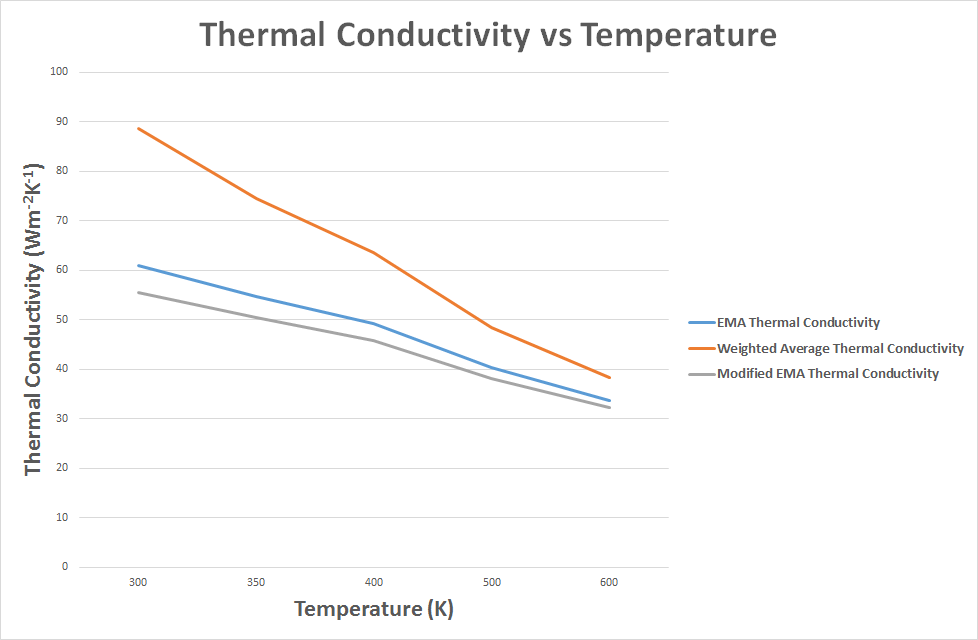
\includegraphics[width=80mm]{kphvstempAM.png}

\subsection{Maximizing Power Factor}
\label{sec:Maximizing Power Factor}


\subsection{Minimizing KT}
\label{sec:Minimizing KT}

\newpage
\begin{thebibliography}{9}
\bibitem{Paper01} \emph{Reference} Source
\end{thebibliography}
\end{document}
